%%%%%%%%%%%%%%%%%%%%%%%%%%%%%%%%%%%%%%%
%%% Corretor numérico
%   Questões práticas sobre o uso do
%   corretor numérico.
%%%%%%%%%%%%%%%%%%%%%%%%%%%%%%%%%%%%%%%
\section{Uso do corretor numérico}\label{secao:uso_do_corretor}
O corretor numérico apresentado na seção \ref{secao:corretor_numerico} possui algumas questões sobre sua usabilidade no programa que valem ser discutidas nesta seção. Para começar, é interessante que o uso de um corretor numérico não eleve drasticamente o tempo necessário para realizar uma simulação. No caso deste corretor, existem alguns custos associados.

O primeiro é no cálculo das integrais primeiras. Embora $\vet \Psi(\vet z_0)$ seja calculado apenas uma vez, a cada iteração que utiliza o corretor é necessário calcular $\vet \Psi(\vet z)$. O cálculo direto da energia total para um potencial de N-corpos, por exemplo, tem ordem $O(N^2)$ de operações, podendo ser então um custo relevante.

Um segundo custo é na resolução do sistema linear (\ref{eq:corretor_equacao_2}), pois a matriz jacobiana $D \vet \Psi$ tem tamanho $k \times 6N$. Observe, porém, que a matriz
\begin{equation}\label{eq:corretor_matriz_normal}
    \vet \Gamma (\vet z) = D \vet \Psi(\vet z) D \vet \Psi(\vet z)^T
\end{equation}
é uma matriz normal, e seu tamanho é $k \times k$. Além disso, cada elemento seu é dado diretamente por um produto interno:
\begin{equation*}
    \vet \Gamma_{ij} = \prodint{\nabla \psi_i}{\nabla \psi_j},
\end{equation*}
o que a caracteriza como uma matriz de Gram, e também em casos com poucas integrais primeiras de interesse isso significa que esta pode ser calculada manualmente, otimizando uma parte do processo. 

Além disso, a resolução do sistema de equações
\begin{equation*}
    \bm \Gamma (\vet y) \vet \alpha = \vet \Psi(\vet z) - \vet \Psi(\vet z_0).
\end{equation*}
também possui um custo associado, o que depende da quantidade de integrais primeiras utilizadas e do método utilizado para resolução. A primeira abordagem computacional tomada foi utilizar a sub-rotina \verb|dgesv|, do LAPACK, a qual resolve um sistema $\bm A \vet x = \vet b$, com $\bm A$ $n \times n$ aplicando a decomposição LU sobre $\bm A$, o que tem custo $O(n^3)$, e resolvendo o sistema triangular restante, com custo $O(n^2)$.

Porém, uma vez que a matriz $\bm \Gamma$ é de Gram, é também no mínimo positiva semi-definida. Isso significa que em vez de utilizar LU, que tem como fundo o pivoteamento gaussiano, faz sentido utilizar a decomposição de Cholesky, que apesar de ter $O(n^3)$ consome apenas metade das operações do pivoteamento gaussiano, e trata-se de um algoritmo que sempre é numericamente estável \citep[172-177]{Trefethen1997}. No LAPACK, as subrotinas utilizadas para isso foram \verb|dpotrf| (para a fatoração de Cholesky) e \verb|dpotrs| (para a resolução de um sistema linear Cholesky-fatorado). 

Realizamos alguns testes com os dois métodos de resolução mas não encontramos diferenças expressivas. Um exemplo de aplicação foi em um problema de $10^3$ corpos com condições de Hénon (ver seção \ref{secao:valores_iniciais}), e o resultado pode ser encontrado na figura \ref{fig:corretor_cholesky_vs_lu_energia} e na tabela \ref{tab:corretor_cholesky_vs_lu_energia}. Vale ressaltar que, quanto ao desempenho, ambas as simulações levaram por volta de 10,4 minutos, com uma pequena vantagem de alguns segundos para o uso de Cholesky.

\begin{figure}
    \centering
    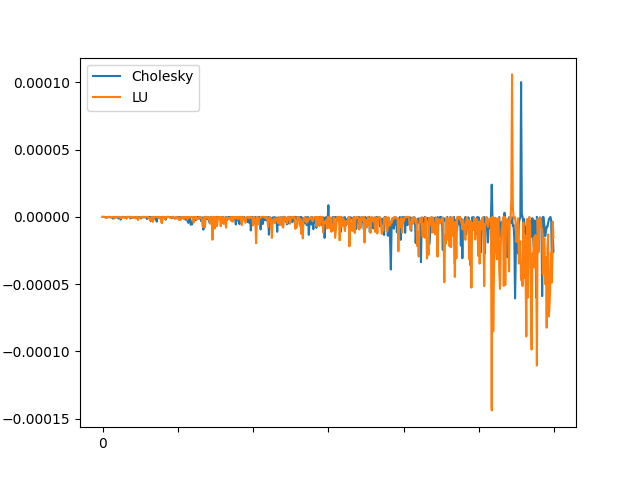
\includegraphics[width=0.5\linewidth]{tcc//img/exemplo_cholesky_vs_lu_energia.png}
    \caption{Variação da energia $\Delta E$ em um problema de $10^3$ corpos utilizando o integrador Velocity-Verlet (2ª ordem), $h=0.1$ e $\epsilon=0.04$, com margem de erro da energia $10^{-11}$.}
    \label{fig:corretor_cholesky_vs_lu_energia}
\end{figure}

\begin{table}[]
    \centering
    \begin{tabular}{c|cc}
                      & Cholesky     & LU           \\ \hline
        Média         & $-3.639 \cdot 10^{-06}$ & $-6.656 \cdot 10^{-06}$ \\
        Mediana       & $-1.208 \cdot 10^{-06}$ & $-1.277 \cdot 10^{-06}$ \\
        Desvio padrão & $8.599 \cdot 10^{-06}$  & $1.551 \cdot 10^{-05}$  
    \end{tabular}
    \caption{Estatísticas sobre o valor $\Delta E$, nas condições da figura \ref{fig:corretor_cholesky_vs_lu_energia}.}
    \label{tab:corretor_cholesky_vs_lu_energia}
\end{table}

Diante do custo, vale questionar também se de fato faz sentido utilizar todas as integrais primeiras no corretor. Por mais que mais informações devam levar a uma correção melhor, uma integral primeira que seja numericamente estável pode ser só um custo a mais e não trazer resultados tão diferentes do que sem o seu uso. 

No PNCG, o centro de massas e o momento linear total são numericamente bem-comportados por serem lineares, e o momento angular também é estável por ser uma expressão livre de singularidades, como exemplificado na figura \ref{fig:var_integrais_es_iau25} da seção \ref{secao:integradores_simpleticos}. A energia total, por outro lado, é bastante instável em aproximações intensas devido ao potencial ser inversamente proporcional às distâncias. Dessa forma, como sugere \cite{Nacozy1972}, aplicar a correção somente na energia total no PNCG é, no geral, suficiente. O vetor de correção $\alpha$ (que é um escalar nesse caso) possui uma forma explícita:
\begin{equation}
    \alpha = \dfrac{E(\vet z) - E(\vet z_0)}{\norma{\nabla E(\vet z)}^2}.
\end{equation}
Um exemplo de aplicação no problema-modelo \ref{probmodelo:iau25} com as duas formas de correção pode ser visualizado na figura \ref{fig:var_energia_iau25_corretores}.

\begin{figure}
    \centering
    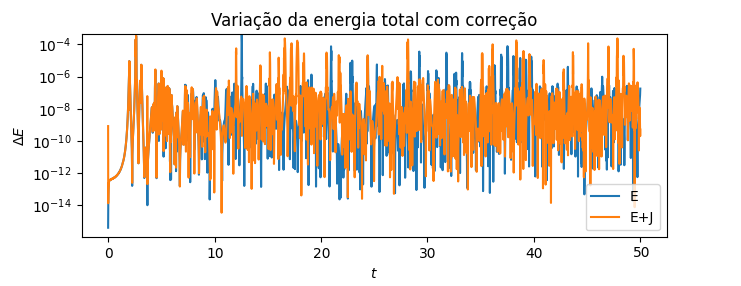
\includegraphics[width=\linewidth]{tcc/img/var_energia_todas_vs_energia_iau25.png}
    % \caption{RKN671 H=0.001, E=0.1, [0,50], COR=1E-10}
    \caption{Variação da energia no problema-modelo \ref{probmodelo:iau25} simulado via método RKN671 com $h=10^{-3}$, $\epsilon = 10^{-1}$ e com margem de erro da energia $10^{-10}$ no intervalo $[0,50]$. Em azul, foi aplicada a correção somente na energia total, enquanto em laranja foi aplicada a correção também no momento angular total.}
    \label{fig:var_energia_iau25_corretores}
\end{figure}

De toda forma, o custo do corretor só ocorre quando este é aplicado, então um bom critério de aplicabilidade pode reduzir o custo do corretor através da sua utilização somente quando estritamente necessário. No problema-modelo utilizado por Nacozy, o corretor era aplicado quando o erro da energia total atingia um valor por volta de 100 vezes menor que o erro de truncamento desejado. Constatamos empiricamente que com o uso do amortecimento no potencial, uma vez que o potencial deixa de ter singularidades, o teto pode ser tanto quanto desejado, então a escolha de Nacozy é razoável para o PNCG.

A implementação do corretor numérico é a sub-rotina \verb|correcao|, que depende de outras sub-rotinas de mecânica do programa.